\chapter{\acro{rtn} Support}

\label{sec:openfstrtn}

%\section{Two Distinct Flavors of \acro{rtn} Support}

% See saprtn.tex.notrack
%Kleene is currently being expanded to provide support for two distinct
%flavors of Recursive Transition Networks or \acro{rtn}s.  This is work in
%progress.

%This section describes the Kleene support for \acro{rtn}s
%compatible with the off-the-shelf functions from the OpenFst library.
%\acro{sap} linguists creating pattern networks for the \acro{sap}
%\acro{rtn} pattern-matching runtime code should ignore this section and
%proceed immediately to section~\ref{sec:saprtn} starting on
%page~\pageref{sec:saprtn}.

\section{OpenFst Recursive Transition Networks (\acro{rtn}s)}

\subsection{Status}

[KRB 2013-04]  WORK IN PROGRESS:  There is currently no runtime-code support for
\init{rtn}s.  This chapter has not be reviewed recently.

Kleene supports the building of Recursive Transition Networks
(\acro{rtn}s) that are compatible with the OpenFst \texttt{Replace()} and
\texttt{ReplaceFst()} operations.  An \acro{rtn} contains arc labels that
are to be interpreted as ``references'' to subnetworks; and compatible
\acro{rtn}-savvy runtime code, when applying a network to data, will
recognize such a reference and ``push'' to the referenced subnetwork to
continue the matching, and then ``pop'' back to the calling network when
the subnetwork has successfully matched.  The references to subnetworks
can also be thought of as non-terminal labels.

\acro{rtn}s, containing references to subnetworks, are often smaller than
full-sized networks that must contain a full copy of each subnetwork
wherever it is needed.  However, \acro{rtn}s can denote context-free
languages, and so can go beyond regular power; a special subclass of
\acro{rtn}s remain regular.  The recognition/parsing of context-free
languages requires memory, in particular a push-down stack, and so any
runtime code to apply \acro{rtn}s must include such a stack.

At the time of writing (13 October 2010) there are hints that the
\acro{rtn} conventions currently required in OpenFst might change, and
there is new library support for mathematically equivalent Pushdown
Automata (\acro{pda}s) that we have not yet tested.  Kleene support for
OpenFst \acro{rtn}s and \acro{pda}s will necessarily evolve along with
the library.

\subsection{Syntax for Creating an OpenFst \acro{rtn}}

For the programmer, there needs to be a Kleene syntax to denote a
reference to a subnetwork, and it needs to be distinct from the syntax
that causes a copy of a network to be inserted.  For example, in this
example

\begin{Verbatim}[fontsize=\small]
$vowel = [aeiou] ;
$net = k $vowel t $vowel b $vowel ;
\end{Verbatim}

\noindent
the \verb!$vowel! network will be copied three times into \verb!$net!.
In real-life applications, a subnetwork might encode something much
larger, such as nouns or even noun phrases in a natural language, and
multiple copies could easily cause the final network to become very
large, or even too large to compute.

Kleene currently supports a wired-in function \verb!$^sub($s)! that
programmers can use to denote a reference to a subnetwork \verb!$s!.\footnote{I'm
not tied to \verb!$^sub($s)! and would be comfortable with alternatives such
as \verb!$^ref($s)! or \verb!$^push($s)!, or even some special syntax like
\verb!>$s<! or \verb!>>$s!.} 

To continue with our trivial example, 

\begin{Verbatim}[fontsize=\small]
$vowel = [aeiou] ;
$rtn = k $^sub($vowel) t $^sub($vowel) b $^sub($vowel) ;
\end{Verbatim}

\noindent
would result in an \verb!$rtn! network that contains three compact
one-label references to \verb!$vowel! rather than three full copies of
it.  In real-life applications, the savings in memory can be very
significant.

\subsection{What does a Reference Look Like in an OpenFst \acro{rtn}?}

OpenFst networks consist of states and arcs, and each arc has two labels,
an input label, and an output label.\footnote{The terminology of
\emph{input} and \emph{output} labels is that of the OpenFst tradition.
In the Xerox tradition, they are called \emph{upper} and \emph{lower}, or
sometimes \emph{lexical} and \emph{surface}.}  In the actual network, the
labels are really integers, and all Unicode characters, such as \emph{a},
\emph{b}, \emph{c}, etc.\@ are represented using their standard Unicode
code point values.  Multichar symbols are stored using code point values
selected at random from a Unicode Private Use Area.

To maximize compatibility with the off-the-shelf OpenFst
\texttt{Replace()} and \texttt{ReplaceFst()} operations, the integer
representing a reference to a subnetwork must currently appear on the
\emph{output} side of an arc.  In Kleene, multichar symbol names
representing a call to a subnetwork \verb!$s! are spelled \verb!__$s!,
with two initial underscores, and the syntax \verb!$^sub($s)!  currently
yields the following network.

% see images/README for converting .ps files to .pdf and cropping them
\begin{center}
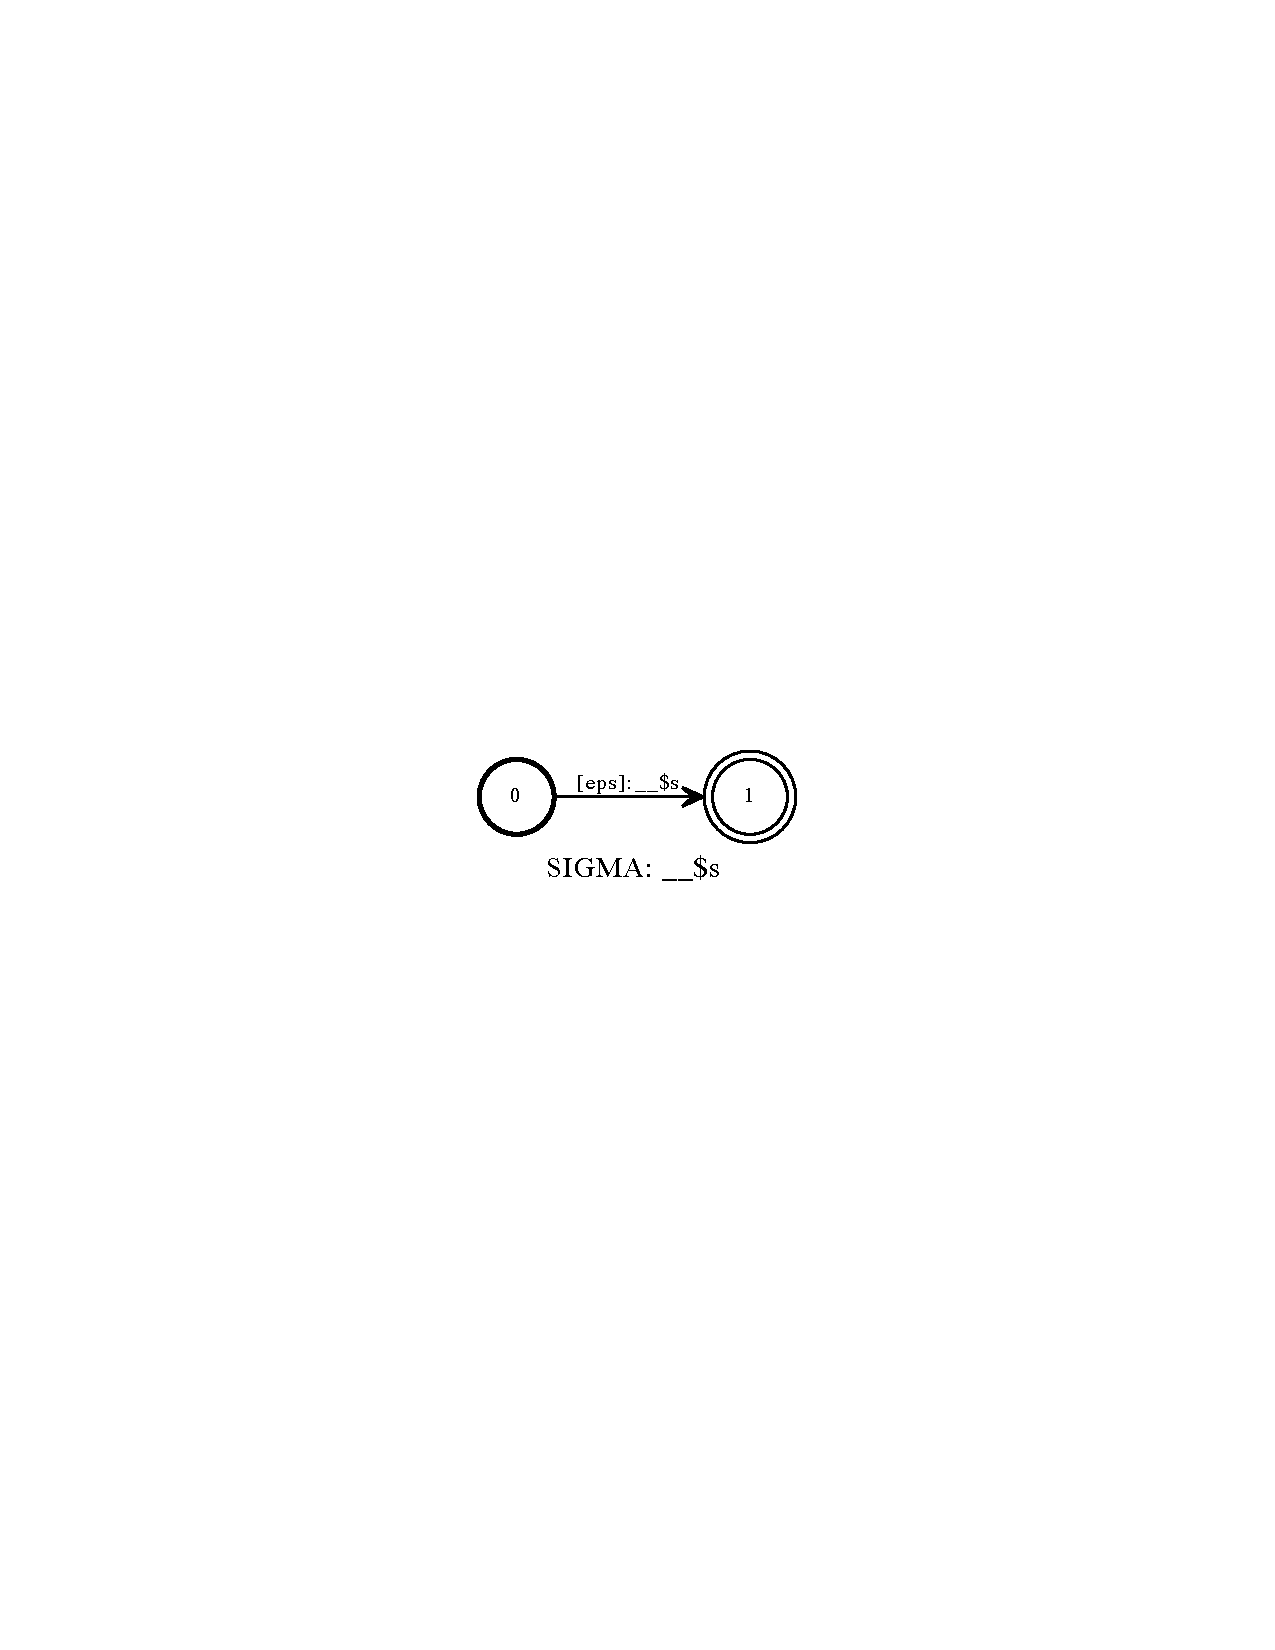
\includegraphics{images/reference.pdf}
\end{center}

\noindent
Currently in OpenFst, the symbol \verb!__$s! could in fact appear also on
the input side.  Of course, in the real network, the labels are really
just integers, 0 for epsilon, and some arbitrary value from the Private
Use Area for the multichar symbol.

Kleene programmers should use the wired-in \verb!$^sub()! function to
denote references to subnetworks and should not try to specify special
symbols like \verb!__$s! directly.  For example, the following statement
is illegal and will cause an exception to be thrown.

\begin{Verbatim}[fontsize=\small]
$rtn = "":'__$foo' ;    // raises an exception
\end{Verbatim}

\noindent
The use of \verb!$^sub()! at the programming level will also make it easy
for Kleene to adapt to any changes to \acro{rtn} representations that
might be made in the underlying OpenFst library.

\subsection{Embedding Subnetworks in an OpenFst \acro{rtn}}

The \verb!$^embedRtnSubnets($rtn)! function takes an OpenFst \acro{rtn}
argument, i.e.\@ a network that contains OpenFst-format references to
subnetworks, and returns a network that consists of the original network
unioned with a prefixed copy of each referred-to subnetwork.  For each
referred-to network \verb!$s!, the prefix consists of the special symbol
\verb!__SUBNETWORKS! followed by the special symbol \verb!__$s!.  Thus
from the following code

\begin{Verbatim}[fontsize=\small]
$p = p ;
$q = q ;
$rtn = a $^sub($p) b $^sub($q) ;
\end{Verbatim}

\noindent
the result \verb!$rtn! is this network containing two references to subnetworks

\begin{center}
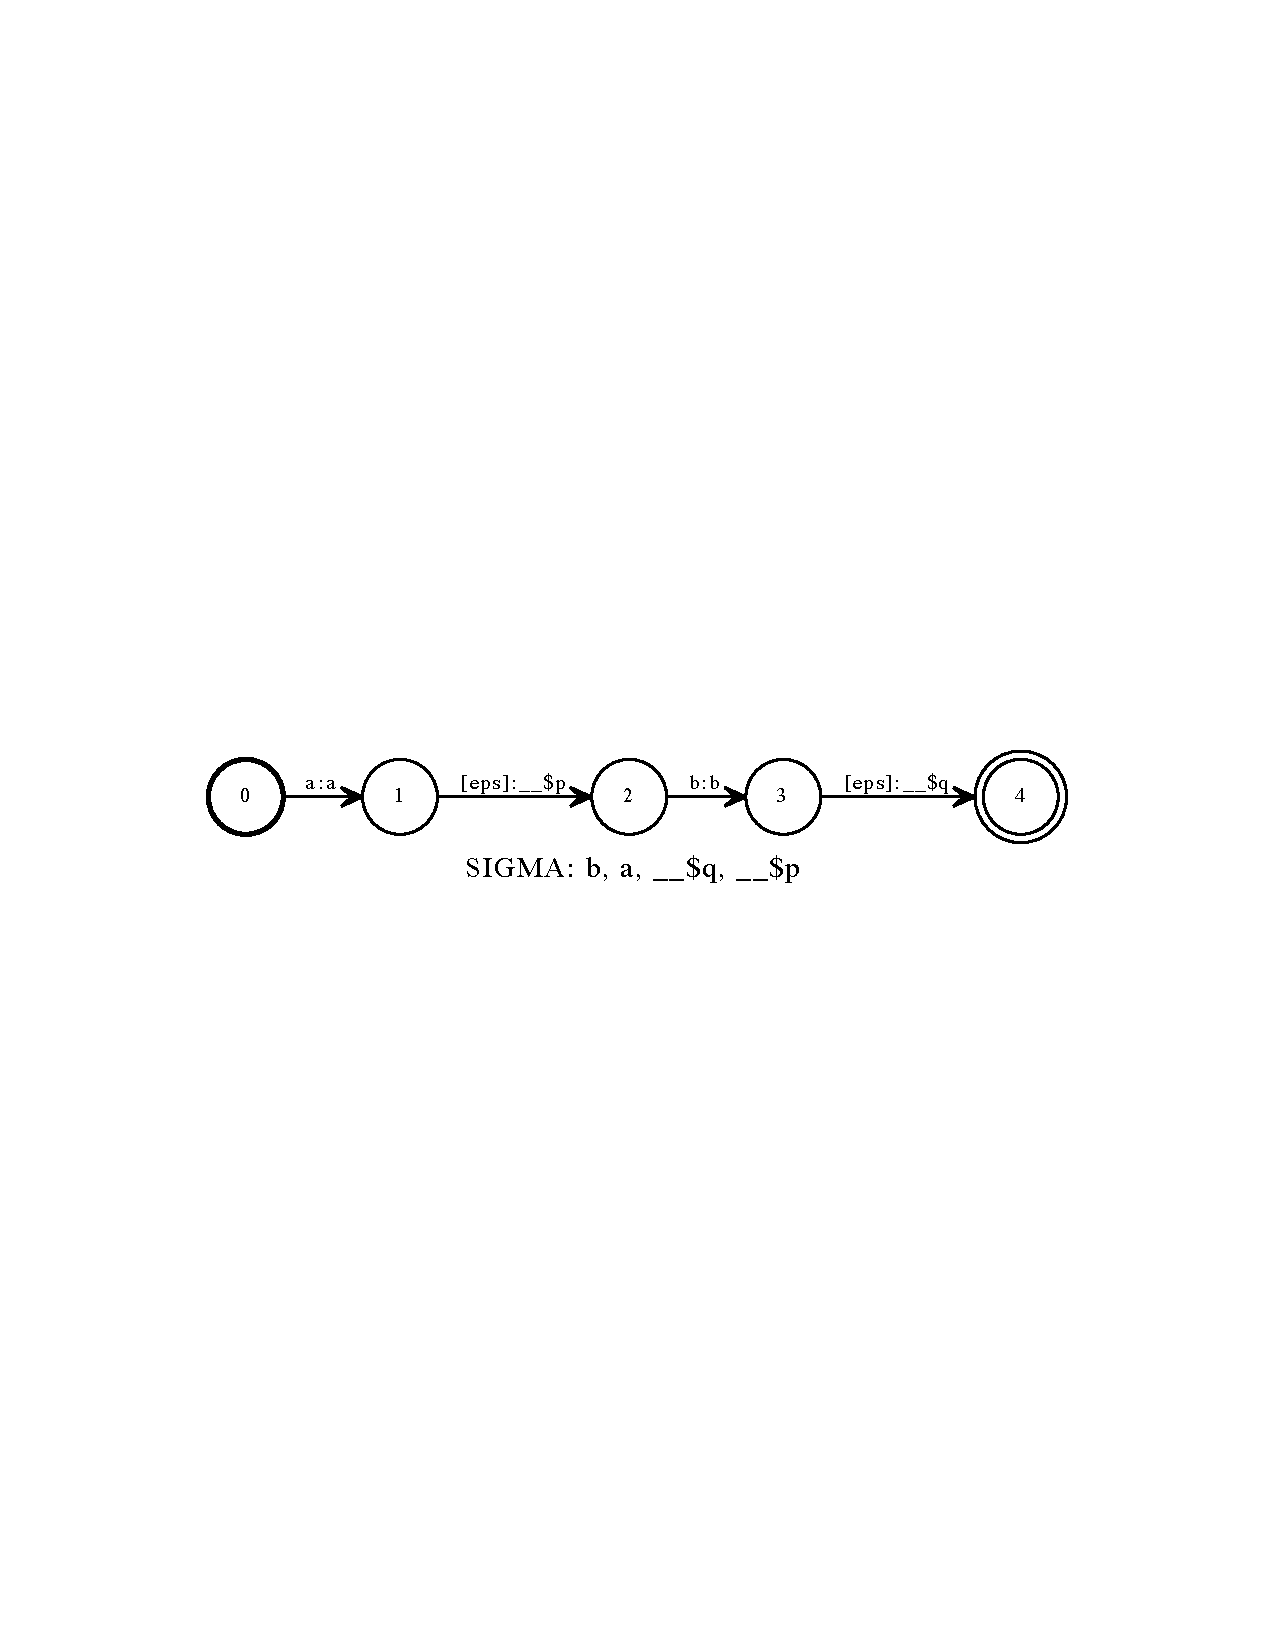
\includegraphics[width=\textwidth]{images/twoReferences.pdf}
\end{center}

\noindent
but the three referred-to networks remain separate.  After the following
call to \verb!$^embedRtnSubnets($rtn)!, 

\begin{Verbatim}[fontsize=\small]
$embedded = $^embedRtnSubnets($rtn) ;
\end{Verbatim}


\noindent
the resulting \verb!$embedded! network looks like this

\begin{center}
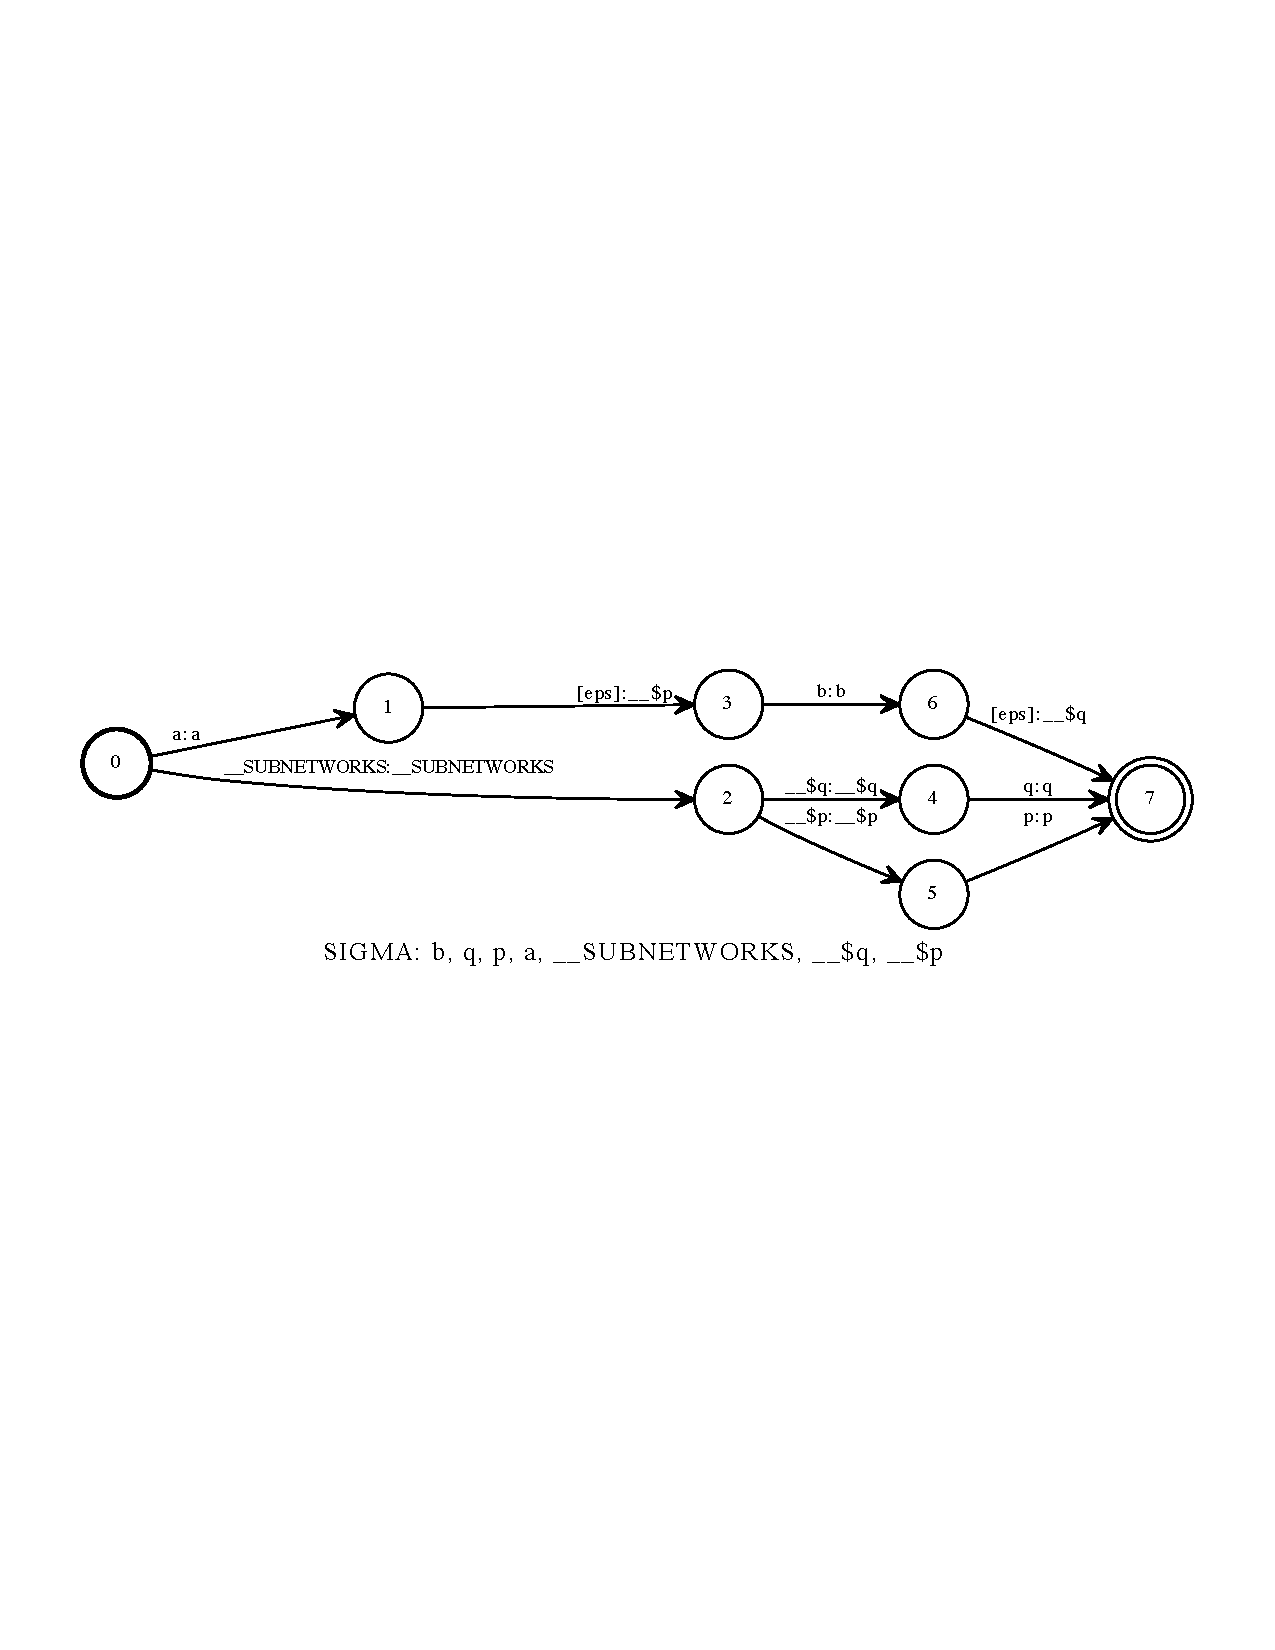
\includegraphics[width=\textwidth]{images/embedded.pdf}
\end{center}

\noindent
The embedded network can be saved to file as a single network and could be
applied by \acro{rtn}-savvy runtime code (not yet written) that knows the prefix convention.

The unioning of the base network with the subnetworks also guarantees that
the meaning of OTHER, if present, is standardized throughout all the
networks.

\subsection{Expanding an OpenFst \acro{rtn} into a Full Normal Network}

In some cases, it may also be useful to take an OpenFst \acro{rtn} and replace
each reference to a subnetwork with an actual copy of that subnetwork,
expanding the \acro{rtn} into a full normal network.  This is mathematically and
computationally possible only if the \acro{rtn} is regular.  Using the same
\verb!$rtn! example, a call to \verb!$^expandRtn()!

\begin{Verbatim}[fontsize=\small]
$expanded = $^expandRtn($rtn) ;
\end{Verbatim}

\noindent
produces the following \verb!$expanded! network

\begin{center}
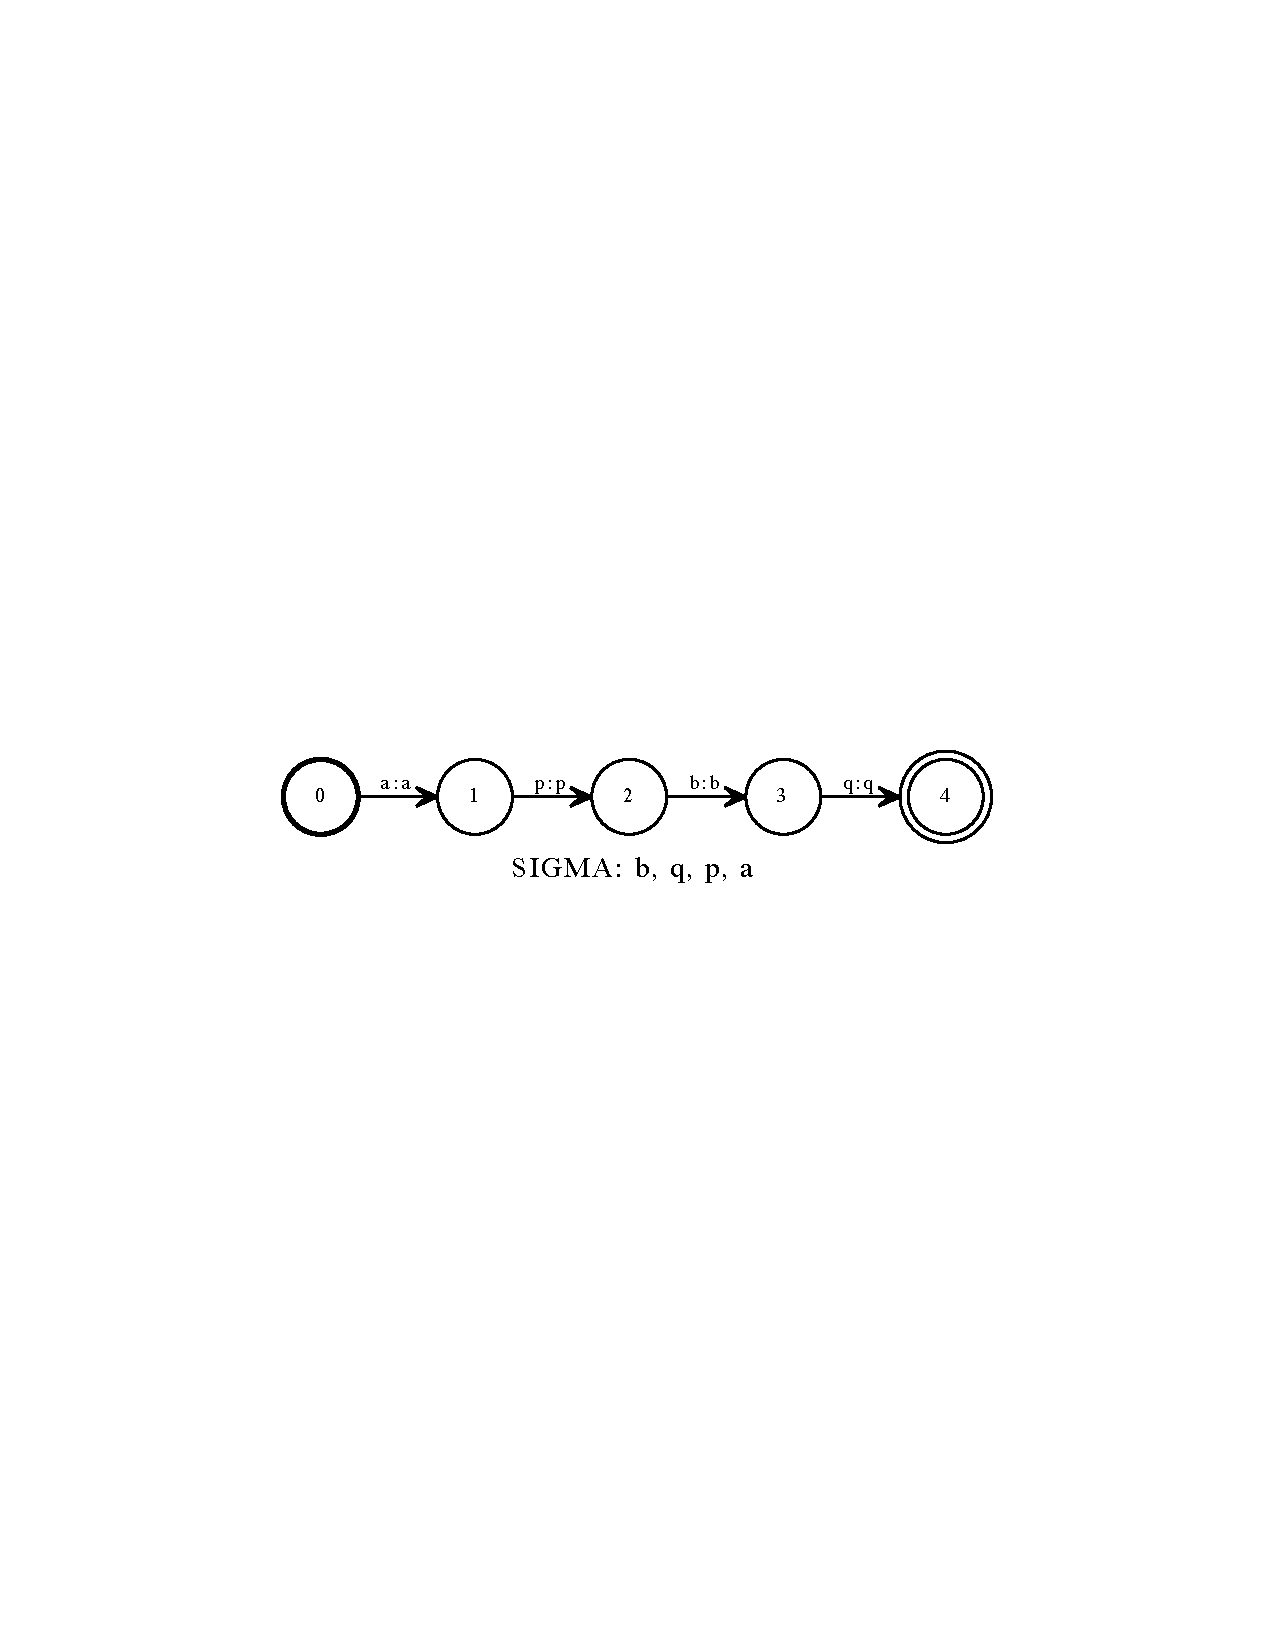
\includegraphics[width=\textwidth]{images/expanded.pdf}
\end{center}

\noindent
In real-life \acro{rtn}s, with multiple references to the same
subnetwork, the expanded network will be significantly bigger than the
original.  

If the \acro{rtn} contains cyclic references to subnetworks, it is
context-free in power (i.e.\@ no longer regular in power), and its
expansion would result in an infinite network.  The
\verb!$^expandRtn($rtn)! function checks for cyclic references and throws
an exception if the \verb!$rtn! is not regular.\footnote{In the OpenFst
library, the \verb!ReplaceFst()! operation provides a convenient method
that checks for cyclic references, and \verb!$^expandRtn()! invokes this
method.}



